\documentclass[a4paper]{article}
\usepackage{amsmath,amssymb,amsfonts,amsthm}
\usepackage{multicol}
\usepackage{multirow}
\usepackage{mathtools}
\usepackage{soul}
\usepackage{hyperref}
\hypersetup{
    colorlinks=true,
    linkcolor=blue,
    filecolor=magenta,      
    urlcolor=cyan,
    pdftitle={Overleaf Example},
    pdfpagemode=FullScreen,
    }
\usepackage{color}
\usepackage[table]{xcolor}
\usepackage[T1]{fontenc}
\usepackage{etoolbox}
\usepackage{multicol}
\usepackage{multirow}
\usepackage{fancyhdr}
\usepackage{graphicx}
\usepackage{array}
\usepackage{amsthm}
\usepackage{titlesec}
\usepackage{tikz}
\usepackage{bm}
\usepackage{enumitem}
\usetikzlibrary{arrows.meta,calc}
\usetikzlibrary{positioning,automata}
\renewcommand{\baselinestretch}{1.2}

\titleformat*{\section}{\large\bfseries}
\titleformat*{\subsection}{\normalsize\bfseries}

\graphicspath{{C:/Users/teoso/OneDrive/Documents/Tugas Kuliah/Template Math Depart/}}

\newtheorem{theorem}{Theorem}
\newtheorem*{teorema}{Teorema}
\newtheorem*{definisi}{Definisi}
\theoremstyle{definition}
\newtheorem*{bukti}{Bukti}
\newtheorem*{solusi}{Solusi}

\newcommand{\Arg}{\text{Arg}}
\newcommand{\trace}{\text{trace}}

\tikzset{->, >=stealth, node distance=3cm, on grid, thick,initial text=,
state/.style={rectangle, rounded corners = 0.35cm, draw, minimum width=1.5cm, minimum height=0.7cm},
every loop/.style={looseness=3}}

\begin{document}
\fancyhead[L]{\textit{Teosofi Hidayah Agung}}
\fancyhead[R]{\textit{5002221132}}
\pagestyle{fancy}
\section*{Exercise 3.1}
\noindent Berikan jejak (traces) pada himpunan proposisi atomik \( \{a, b\} \) dari sistem transisi berikut:
\begin{center}
  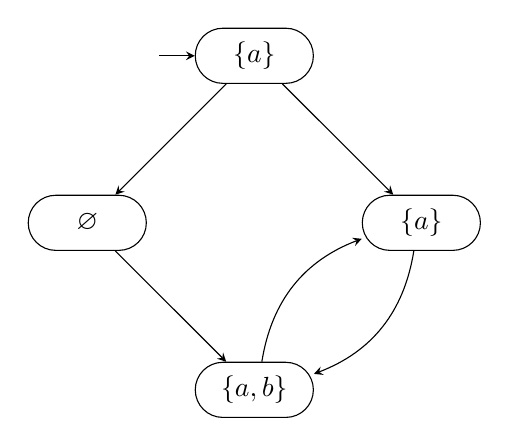
\begin{tikzpicture}

    % Nodes
    \node[state, initial] (q1) { $\{a\}$ };
    \node[state, below left=of q1] (q2) { $\varnothing$ };
    \node[state, below right=of q2] (q3) { $\{a, b\}$ };
    \node[state, below right=of q1] (q4) { $\{a\}$ };

    % Edges
    \path (q1) edge node {} (q2)
          (q1) edge node {} (q4)
          (q2) edge node {} (q3)
          (q3) edge[bend left] node {} (q4)
          (q4) edge[bend left] node {} (q3);
  \end{tikzpicture}
\end{center}

\begin{solusi}
  Perhatikan bahwa traces dari \textit{path} dimulai dari \(\{a\}\) dan akan menuju antara \(\varnothing\) atau \(\{a, b\}\). Selanjutnya, kedua \textit{path} tersebut akan berlanjut ke \(\{a, b\}\) dan terjadi sebuah \textit{loop} antara \(\{a\}\) dan \(\{a, b\}\). Dengan demikian, traces dari sistem transisi tersebut hanya ada dua, yaitu:
  \begin{enumerate}
    \item \(\trace(\pi_1)=\{a\}\, \varnothing\, \{a, b\}\, \{a\}\, \{a, b\}\, \{a\}\, \{a, b\}\, \{a\}\, \{a, b\}\, \ldots\)
    \item \(\trace(\pi_2)=\{a\}\, \{a\}\, \{a, b\}\, \{a\}\, \{a, b\}\, \{a\}\, \{a, b\}\, \{a\}\, \{a, b\}\, \ldots\)
  \end{enumerate}
\end{solusi}

\section*{Exercise 3.5}
\noindent Perhatikan himpunan \( AP \) dari proposisi atomik yang didefinisikan oleh 
\( AP = \{ x = 0, x > 1 \} \) dan pertimbangkan sebuah program komputer \( P \) yang berjalan tanpa henti 
dan memanipulasi variabel \( x \). Nyatakan properti-properti berikut, yang dinyatakan secara informal, dalam bentuk properti LT:

\begin{enumerate}
    \item salah
    \item pada awalnya, \( x \) bernilai nol
    \item pada awalnya, \( x \) tidak bernilai nol
    \item pada awalnya, \( x \) bernilai nol, tetapi pada suatu titik \( x \) melebihi satu
    \item \( x \) melebihi satu hanya dalam jumlah terbatas
    \item \( x \) melebihi satu dalam jumlah tak hingga kali
    \item nilai \( x \) bergantian antara nol dan dua
    \item benar
\end{enumerate}

\begin{solusi}
  $\,$
  \begin{enumerate}
    \item[(a)] $P_{\text{false}} = \varnothing$ \\ (Selalu salah)
    
    \item[(b)] Awalnya, $x$ sama dengan nol:
    \[
    P=\{A_0A_1A_2\dots\,|\,(x=0)\in A_0\}
    \]
    
    \item[(c)] Awalnya, $x$ berbeda dari nol:
    \[
    P=\{A_0A_1A_2\dots\,|\,(x=0)\notin A_0\}
    \]

    \item[(d)] Awalnya, $x$ sama dengan nol, tetapi pada suatu saat $x$ melebihi satu:
    \[
    P=\{A_0A_1A_2\dots\,|\,(x=0)\in A_0\land\exists n>0,(x>1)\in A_n\}
    \]

    \item[(e)] $x$ melebihi satu hanya dalam jumlah terbatas:
    \[
    P=\{A_0A_1A_2\dots\,|\,\exists n>0,(x>1)\in A_n\land\exists M,\forall i>M,(x> 1)\notin A_i\}
    \]

    \item[(f)] $x$ melebihi satu dalam jumlah tak hingga:
    \[
    P=\{A_0A_1A_2\dots\,|\,\forall i>0\,\exists N>i, (x>1)\in A_N\}
    \]

    \item[(g)] Nilai $x$ bergantian antara nol dan dua:
    \[
    P=\{A_0A_1A_2\dots\,|\,\forall i\geq 0,A_{i}\in\{x=0,x>1\}\land A_{i}\ne A_{i+1}\}
    \]

    \item[(h)] $P_{\text{true}}=(2^{AP})^\omega$\\
    (Selalu benar)
  \end{enumerate}
\end{solusi}
  
\end{document}